\chapter{Anàlisi final del treball}
\section{Implementació del treball a la FPGA}
\par Finalment, es sintetitzen els blocs documentats en els apartats anteriors i es tracen les connexions necessàries en el diagrama de blocs del projecte de Vivado. El diagrama final es pot veure a l'annex 5. S'adjunten els resultats en l'utilització dels recursos de la FPGA a la taula \ref{taula_recursosFPGA} i l'informe del timing dels processos (\ref{figTiming}) a la FPGA juntament amb el dels consums de potència (\ref{figPWR}).
\begin{figure}[H]
    \centering
    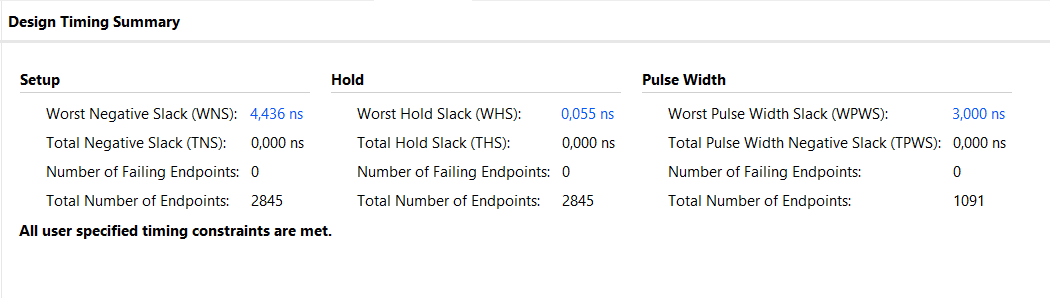
\includegraphics[width=0.6\linewidth]{Images/Timingreport.png}
    \caption{Informe del timing dels processos dins la FPGA.}
    \label{figTiming}
\end{figure}
\begin{figure}[H]
    \centering
    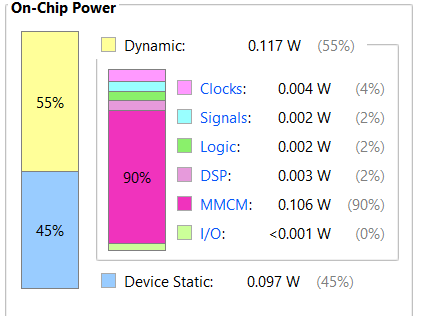
\includegraphics[width=0.4\linewidth]{Images/PWR_FPGA.png}
    \caption{Informe dels consums de potència dels subprocessos en la implementació a la FPGA.}
    \label{figPWR}
\end{figure}
\begin{table}
    \centering
    \begin{tabular}{ | c | c | }
    \hline
    \textbf{Recurs}     &  \textbf{Nombre}\\ [2ex] 
    \hline
    LUTs     &  1170\\
    \hline
    Registres     &  891\\
    \hline
    Slices     &  247\\
    \hline
    Muxes     &  46\\
    \hline
    DSPs     &  4\\
    \hline
    \end{tabular}
    \caption{Utilització de recursos de la FPGA en la implementació final del projecte.}
    \label{taula_recursosFPGA}
\end{table}

\par A la figura \ref{figTiming} es pot observar que el projecte sintetitzat compleix amb els requeriments dels temps de setup dels blocs síncrons, amb un marge positiu de +4,436 ns respecte al temps de setup més crític. Per tant, el sistema no presenta risc de metaestabilitat als blocs interns de la FPGA. En lo referent al consum de la implementació del projecte a la FPGA, el bloc que consumeix més potència és el bloc de gestió del rellotge de la FPGA i només consumeix 100 mW. Per últim, el disseny consumeix menys d'1\% del total dels recursos disponibles del model Artix-7 (\ref{taulaArtix7}).

\section{Resultats experimentals}
\par Per poder validar el projecte implementat, s'ha analitzat la resposta del sistema a una entrada sinusoidal de 1 kHz de freqüència. S'ha utilitzat un arxiu .wav de la sinusoidal samplejada a 44.1 kHz i d'amplada 16 bits \cite{Sin1kHZ} per transmetre-la des de la font d'àudio pel bus I2S i s'ha capturat la sortida PDM i la sortida analògica en un oscil·loscopi.
\begin{figure}[H]
    \centering
    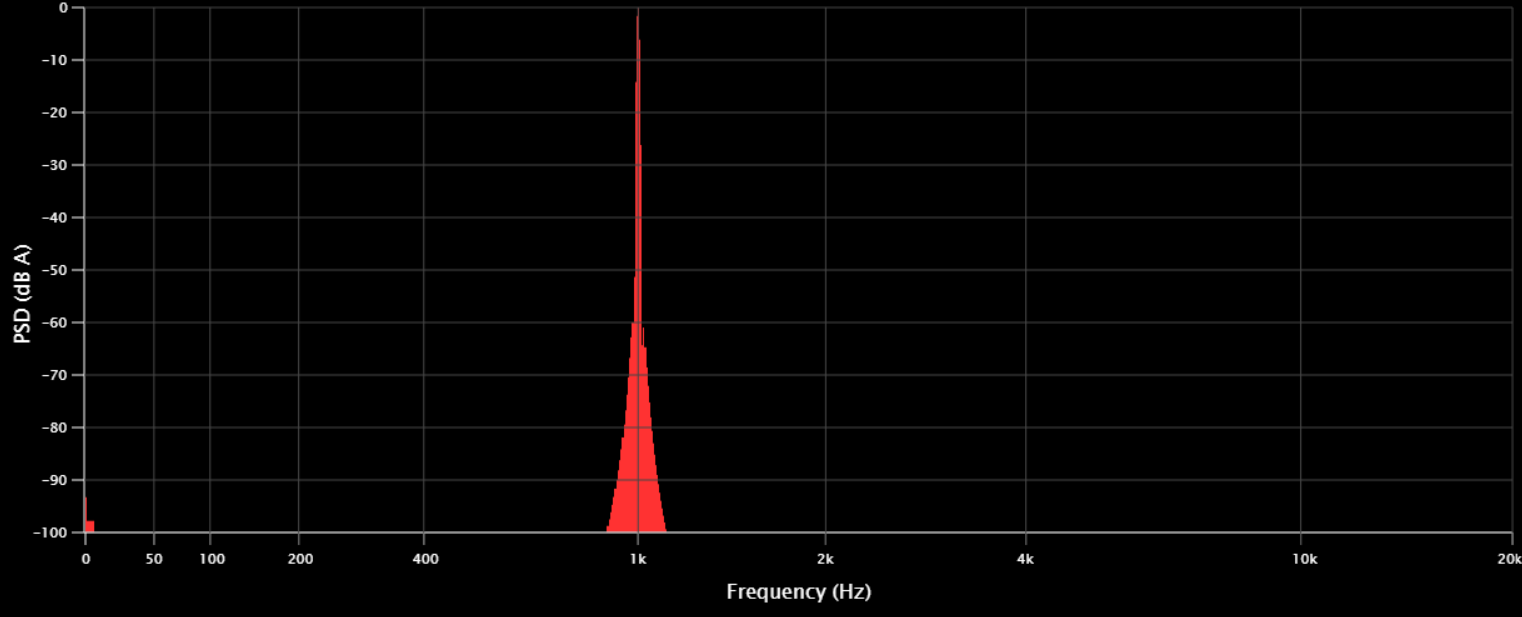
\includegraphics[width=0.7\linewidth]{Images/FFT_in.png}
    \caption{FFT del senyal sinusoidal de 1 kHz a l'entrada.\cite{FFTSin1kHz}}
    \label{figFFTsine}
\end{figure}
\par A la figura \ref{figFFT_tot} es pot observar com la FFT del senyal de sortida en format PDM no és del tot nítida i té una arrissada apreciable en tot l'espectre. A la figura \ref{figPDM_gran}, es pot visualitzar la trama PDM i intuir l'amplada dels respectius polsos.  
\par D'altra banda, la FFT de la sortida analògica es mostra a la figura \ref{figFFT_1kHz} i \ref{fig_FFT2kHz}, on es pot apreciar que el senyal fonamental de 1 kHz té una amplitud similar a la de l'harmònic de 2,5 kHz. Possibles fonts de soroll poden ser la mala connexió de la sonda a l'hora de capturar els senyals i la presència d'elements paràsits en la implementació del test. En conjunt, és plausible que totes les fonts de soroll mencionades influeixin al senyal, reproduint la sortida d'àudio lleugerament distorsionada. 
\par En conclusió, el sistema és capaç de transmetre un senyal d'àudio reconeixible, però amb soroll acoblat a la sortida. En la realització d'aquest treball, no ha donat temps a dissenyar una etapa que ataqui aquesta problèmatica mencionada. 

\begin{figure}
    \centering
    \includegraphics[width=0.5\linewidth]{Images/Setup_test.png}
    \caption{Setup del test pràctic per a la validació final del sistema implementat.}
    \label{figsetup}
\end{figure}

\newpage

\begin{figure}[H]
    \centering
    \includegraphics[width=0.5\linewidth]{Images/FFT_tot.png}
    \caption{FFT de la sortida PDM del sistema.}
    \label{figFFT_tot}
\end{figure}

\begin{figure}[H]
    \centering
    \includegraphics[width=0.5\linewidth]{Images/FFT_1kHz.PDMpng.png}
    \caption{FFT de la sortida PDM del sistema, amb el cursor sobre la freqüència de 1 kHz i 1 MHz.}
    \label{figFFT1kPDM}
\end{figure}

\begin{figure}[H]
    \centering
    \includegraphics[width=0.5\linewidth]{Images/FFT_8kHz.png}
    \caption{FFT de la sortida PDM del sistema, amb el cursor sobre la freqüència de 8,76 kHz i 1 MHz.}
    \label{figFFT8kPDM}
\end{figure}

\begin{figure}[H]
    \centering
    \includegraphics[width=0.5\linewidth]{Images/FFT_5kHz.png}
    \caption{FFT de la sortida PDM del sistema, amb el cursor sobre la freqüència de 5 kHz i 1 MHz.}
    \label{figFFT5kPDM}
\end{figure}

\begin{figure}[H]
    \centering
    \includegraphics[width=0.5\linewidth]{Images/PDM_outgran.png}
    \caption{Trama de la sortida PDM del sistema.}
    \label{figPDM_gran}
\end{figure}

\begin{figure}[H]
    \centering
    \includegraphics[width=0.5\linewidth]{Images/FFT_1kHz.png}
    \caption{FFT de la sortida analògica del sistema, centrat a l'origen de coordenades la freqüència de 1 kHz.}
    \label{figFFT_1kHz}
\end{figure}

\begin{figure}[H]
    \centering
    \includegraphics[width=0.5\linewidth]{Images/FFT_2kHz.png}
    \caption{FFT de la sortida analògica del sistema, centrat a l'origen de coordenades la freqüència de 2,5kHz.}
    \label{fig_FFT2kHz}
\end{figure}

\section{Valoració final dels objectius}
Per concloure la realització d'aquest treball, es recuperen els objectius establerts a l'introducció i es fa una valoració de si s'han complert i de les problemàtiques enfrontades.  

\subsubsection{Objectiu 1}
\begin{quote}
    \textit{Implementar un bloc IP receptor per fer lectures en protocol I2S.}
\end{quote}
\par El primer objectiu s'ha assolit de forma satisfactòria, ja que s'ha pogut implementar un bloc IP d'un receptor del protocol I2S. L'entitat receptora I2S s'ha dissenyat íntegrament en codi VHDL i amb una arquitectura estructural. Com s'ha pogut demostrar al capítol 4, el bloc captura correctament les trames d'àudio que es transmeten pel bus i les guarda al registre de sortida. 
\par No obstant, la validació empírica del bloc ha estat condicionada per la font d'àudio ja que aquesta inicialment no era capaç de transmetre informació pel bus I2S.   

\subsubsection{Objectiu 2}
\begin{quote}
    \textit{Dissenyar i implementar etapes de filtrat per l'àudio a l'entrada i sobremostrejar el senyal.}
\end{quote}
\par El segon objectiu s'ha implementat correctament fent ús dels blocs IP LogiCORE CIC Compiler i FIR Compiler, i configurant-los per complir les especificacions de disseny. 
\par Per contra, l'implementació d'aquesta etapa ha tardat més temps de l'esperat retrassant les altres fases de disseny. Inicialment, es va optar per descriure el procés de filtrat i interpolació en codi VHDL però no es van acabar de resoldre les derives en l'estabilitat del sistema. Finalment es va dessistir en el desenvolupament del codi en VHDL, a favor de completar la realització del treball. 

\subsubsection{Objectiu 3}
\begin{quote}
    \textit{Dissenyar i implementar un modulador $\Sigma \Delta$ que modeli el soroll provocat per la quantificació.}
\end{quote}
\par S'ha complert el tercer objectiu, implementant un modulador $\Sigma \Delta$ de segon ordre. L'entitat s'ha pogut descriure en VHDL al complet, aplicant una modelació del soroll de quantificació efectiva. 
\par En canvi, no s'ha aconseguit implementar un modulador d'ordre superior perquè no s'ha pogut garantir l'estabilitat del sistema. La implementació de moduladors $\Sigma \Delta$ amb més de dos blocs integradors no es pot dur a terme de manera directa, com en el cas d'un modulador de segon ordre, ja que cal considerar la re-ubicació dels nous pols en el sistema per assegurar-ne l'estabilitat. 

\subsubsection{Objectiu 4}
\begin{quote}
    \textit{Dissenyar una etapa de delmat del senyal d'àudio provinent del bloc $\Sigma \Delta$.}
\end{quote}
\par No s'ha pogut assolir el quart objectiu degut a la falta de temps per poder dedicar-li el temps necessari per a la implementació. Momentàneament es va intentar implementar un etapa de filtrat austera amb un bloc IP FIR Compiler, pero malauradament no va funcionar. D'haver fet una gestió més eficient del temps en la realització d'aquest treball, hagués sigut possible dissenyar una etapa de filtrat específica pel senyal en format PDM, a la sortida del bloc $\Sigma \Delta$.